% "{'classe':('PSI'),'chapitre':'chs_leq','type':('application'),'titre':'Mât réacteur A320', 'source':'F. Weiss','comp':['B2-15','CHS-01','CHS-02'],'corrige':True}"
%\setchapterimage{bandeau}
\chapter*{Application \arabic{cptApplication} :\\ 
Mât réacteur A320 -- \ifprof Corrigé \else Sujet \fi}
\addcontentsline{toc}{section}{Application \arabic{cptApplication} : Mât réacteur A320 -- \ifprof Corrigé \else Sujet \fi}

\iflivret \stepcounter{cptApplication} \else
\ifprof  \stepcounter{cptApplication} \else \fi
\fi

\setcounter{question}{0}
\marginnote{D'après F. Weiss.}
\marginnote[1cm]{
\UPSTIcompetence[2]{B2-15}
}


 L’étude porte sur la solution d’assemblage choisie entre le mât-réacteur et l’aile de l’avion A320. Les figures suivantes présentent les différentes pièces de cet assemblage ainsi que la disposition des liaisons dans le plan $(\vect{X}, \vect{Z})$.
 
 
\begin{figure*}[!h]
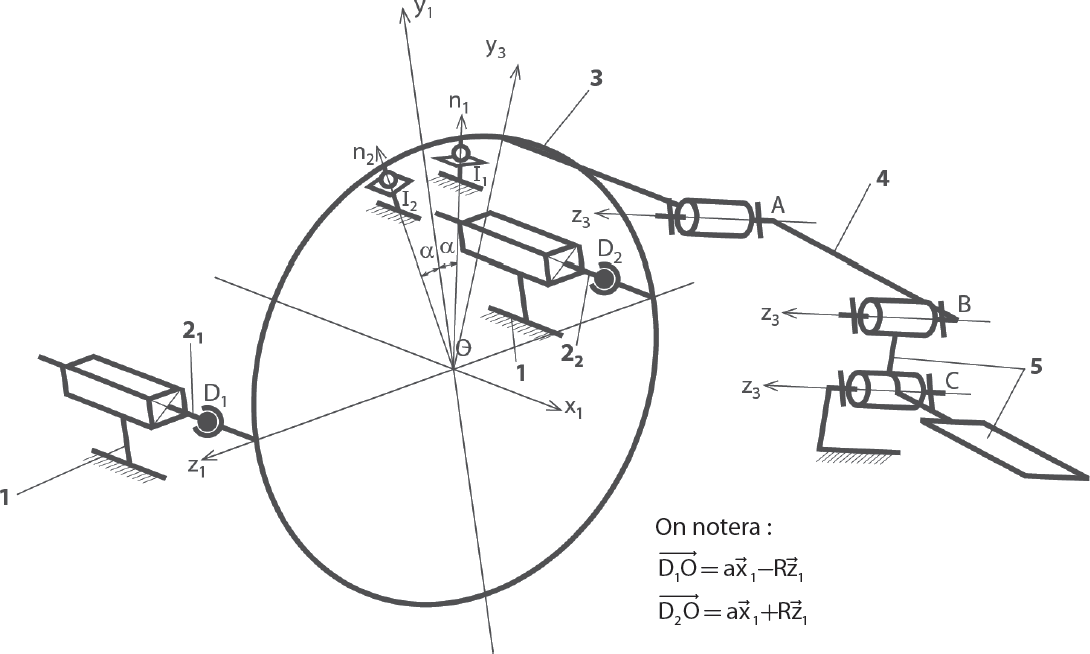
\includegraphics[width=.45\linewidth]{fig_05}
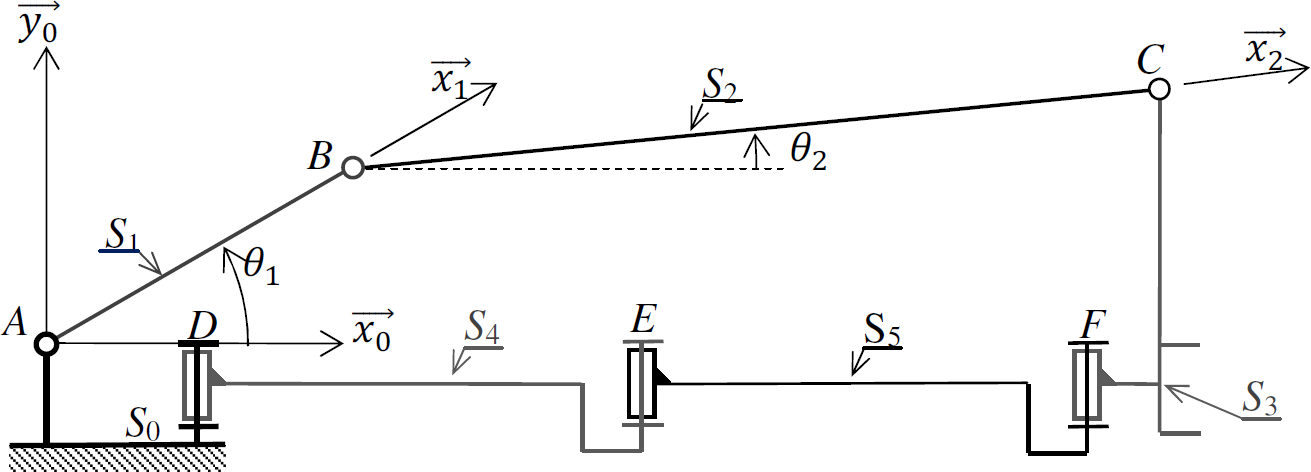
\includegraphics[width=.45\linewidth]{fig_06}
\end{figure*}

Le mât-réacteur \textbf{(1)} est suspendu à l’aile \textbf{(0)} grâce aux deux biellettes \textbf{(4)} et \textbf{(5)}.
Les articulations réalisées aux points $A$, $B$, $N$ et $M$ sont considérées comme des liaisons << sphériques >>. On a : $\vect{AM}=\vect{BN}=a\vect{z}$ .
Les mouvements du mât-réacteur \textbf{(1)} par rapport à l’aile \textbf{(0)} sont stoppés par la présence de deux triangles \textbf{(2)} et \textbf{(3)}. Le triangle \textbf{(2)} est articulé sur \textbf{(1)} par deux liaisons « shériques » de centres $E$ et $F$, et sur \textbf{(0)} par une liaison « sphérique » de centre $H$. On a : $\vect{EF}=e\vect{y}$ et $\vect{EH}=\dfrac{1}{2}e\vect{y}+h\vect{z}$.

Le triangle \textbf{(3)} est articulé sur \textbf{(1)} par deux liaisons « shériques » de centres $C$ et $D$, et sur \textbf{(0)} par une liaison « sphérique » de centre $J$. On a : $\vect{CD}=a\vect{y}$  et  $\vect{CJ}=\dfrac{1}{2}c\vect{y}-j\vect{x}$.

\question{Tracer le graphe de structure de l’assemblage.}

\question{Déterminer la liaison équivalente entre \textbf{(1)} et \textbf{(0)} réalisée par la biellette \textbf{(4)} puis par la biellette \textbf{(5)}.}

\question{Déterminer la liaison équivalente réalisée entre \textbf{(1)} et \textbf{(0)} par le triangle \textbf{(2)} puis par le triangle \textbf{(3)}.}

\question{Tracer en perspective le schéma architectural de l’assemblage du mât \textbf{(1)} sur l’aile \textbf{(0)} en utilisant les modèles des liaisons équivalentes déterminées aux questions précédentes.}

\question{Déterminer le degré d’hyperstatisme de l’assemblage \textbf{(1)}/\textbf{(0)} ; justifier l’intérêt du résultat en raisonnant sur les dilatations provoquées par des températures et des matériaux différents pour l’aile et le mât-réacteur.}


\ifprof
\else
\begin{marginfigure}
\centering

\includegraphics[width=3cm]{Cy_06_01_Application_03_MatReacteur_qr}
\end{marginfigure}
\fi


\ifprof
 
\begin{center}
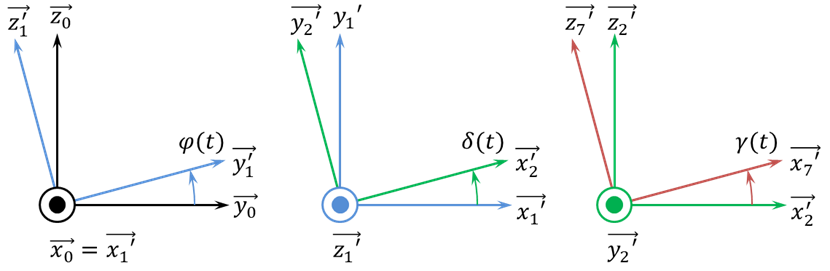
\includegraphics[width=.7\linewidth]{cor_01}
\end{center}

\begin{center}
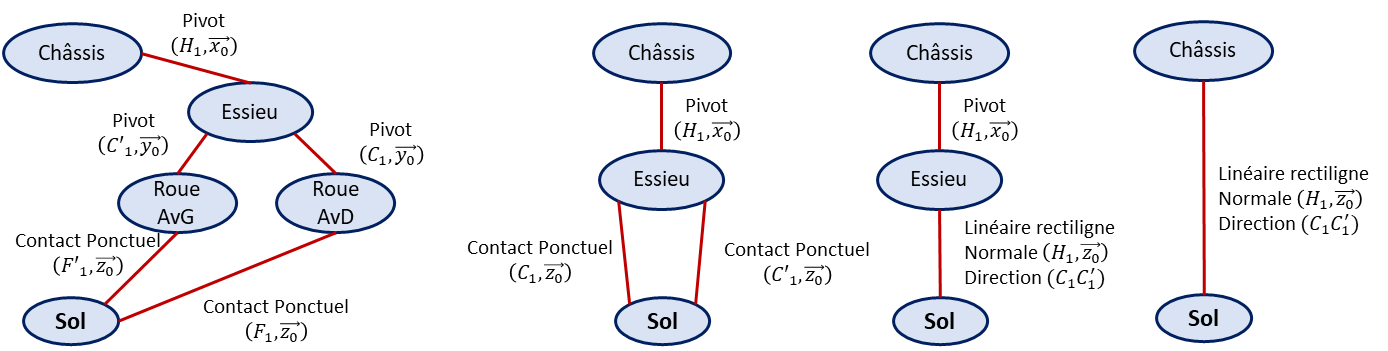
\includegraphics[width=.95\linewidth]{cor_02}
\end{center}

\begin{center}
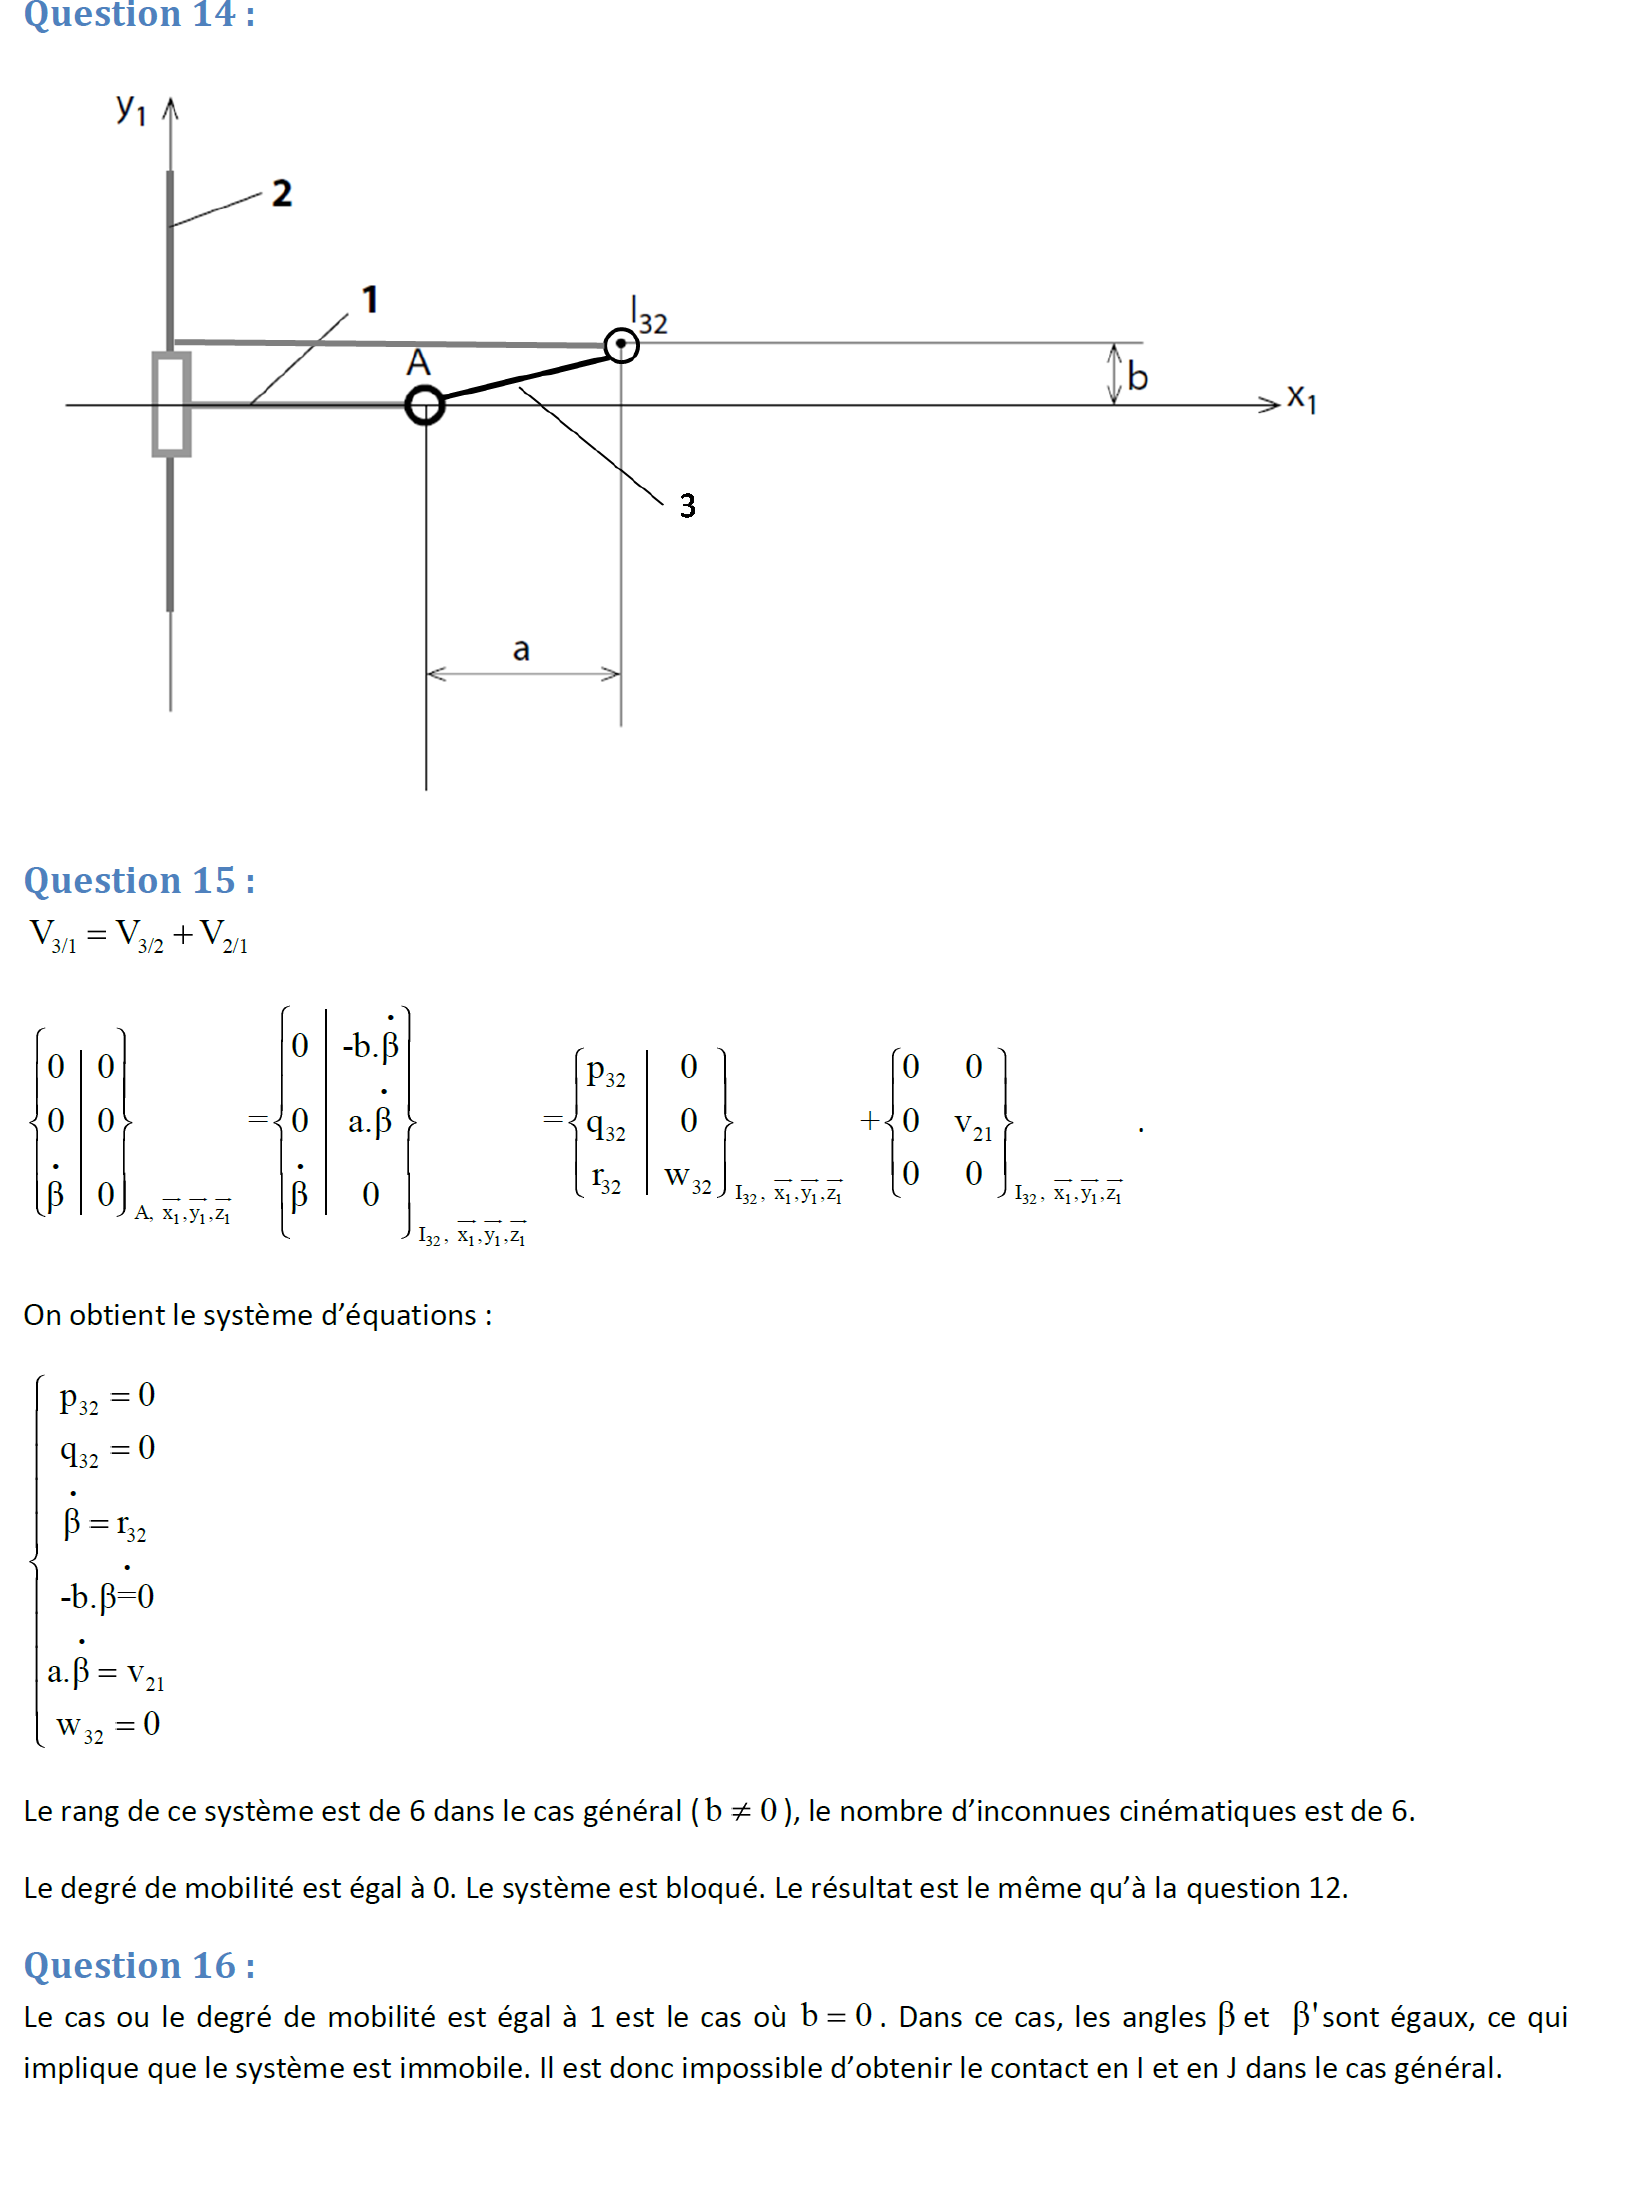
\includegraphics[width=.95\linewidth]{cor_03}
\end{center}

\begin{center}
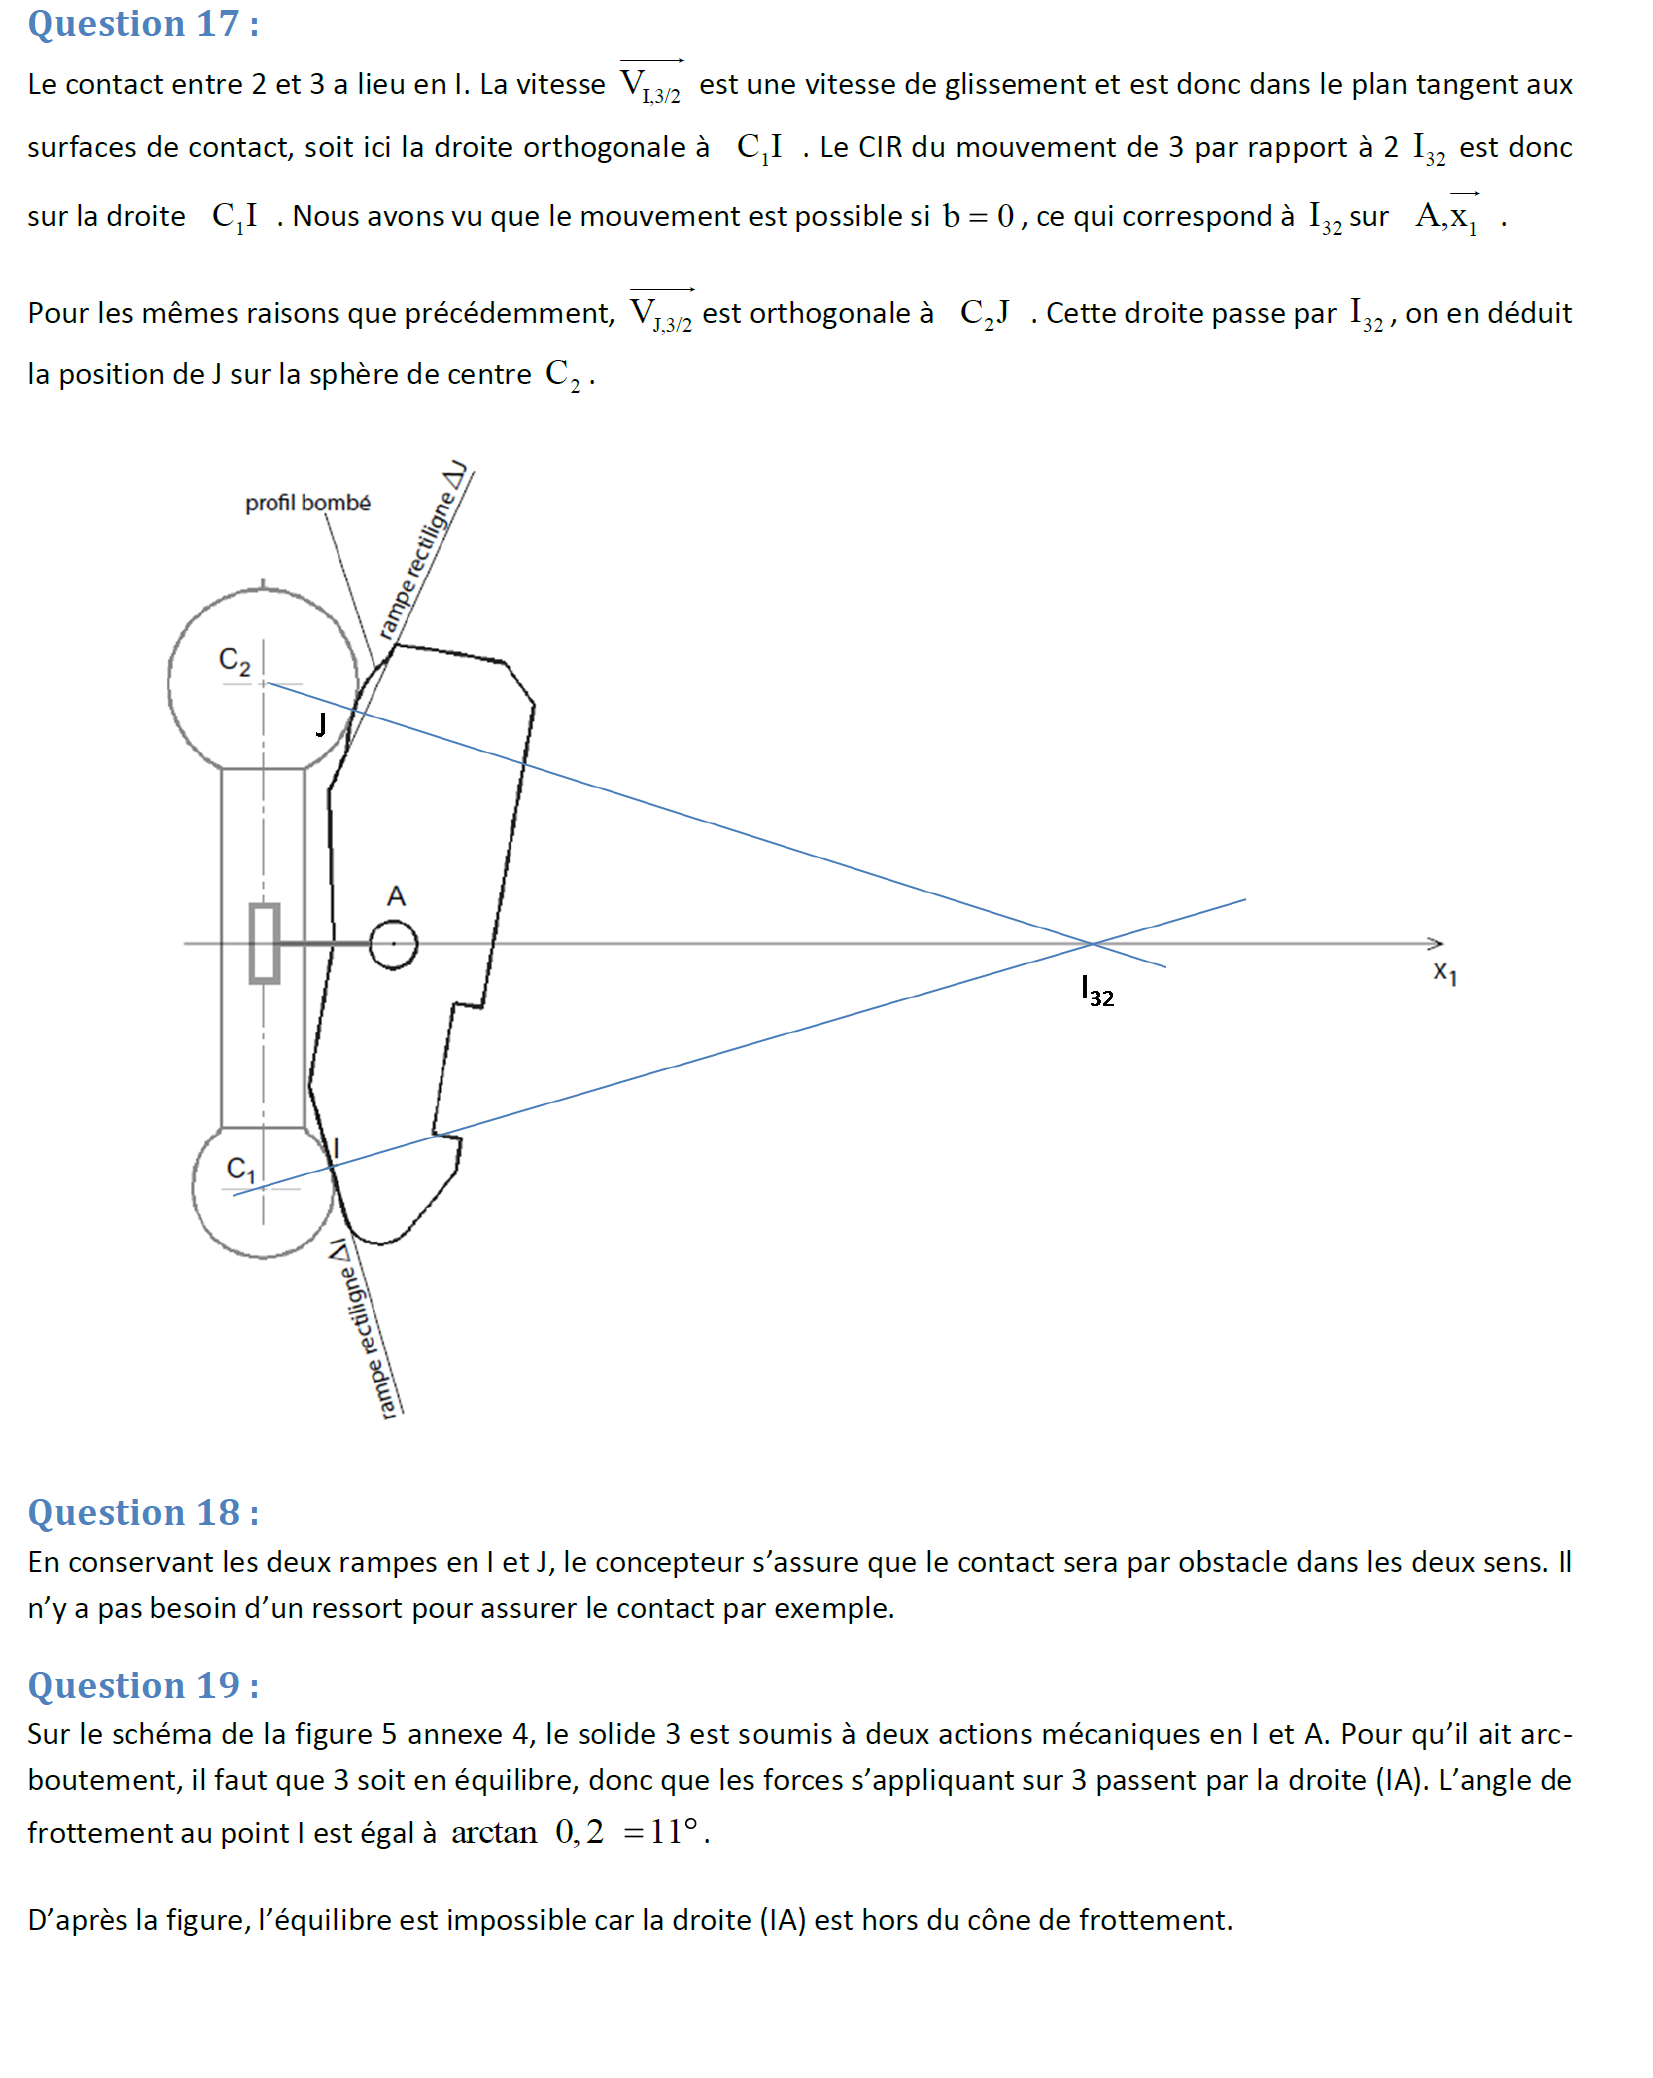
\includegraphics[width=.95\linewidth]{cor_04}
\end{center}

\else
\fi